%  A simple AAU report template.
%  2015-05-08 v. 1.2.0
%  Copyright 2010-2015 by Jesper Kjær Nielsen <jkn@es.aau.dk>
%
%  This is free software: you can redistribute it and/or modify
%  it under the terms of the GNU General Public License as published by
%  the Free Software Foundation, either version 3 of the License, or
%  (at your option) any later version.
%
%  This is distributed in the hope that it will be useful,
%  but WITHOUT ANY WARRANTY; without even the implied warranty of
%  MERCHANTABILITY or FITNESS FOR A PARTICULAR PURPOSE.  See the
%  GNU General Public License for more details.
%
%  You can find the GNU General Public License at <http://www.gnu.org/licenses/>.
%
%  A simple AAU PhD thesis template (collection of papers).
%  2013-05-26 v. 1.1.0
%  Copyright 2012-2013 by Jesper Kjær Nielsen <jkn@es.aau.dk>
%
%  This is free software: you can redistribute it and/or modify
%  it under the terms of the GNU General Public License as published by
%  the Free Software Foundation, either version 3 of the License, or
%  (at your option) any later version.
%
%  This is distributed in the hope that it will be useful,
%  but WITHOUT ANY WARRANTY; without even the implied warranty of
%  MERCHANTABILITY or FITNESS FOR A PARTICULAR PURPOSE.  See the
%  GNU General Public License for more details.
%
%  You can find the GNU General Public License at <http://www.gnu.org/licenses/>.
%
\documentclass[10pt,twoside,b5paper,openright]{book}
%%%%%%%%%%%%%%%%%%%%%%%%%%%%%%%%%%%%%%%%%%%%%%%%
% Language, Encoding and Fonts
% http://en.wikibooks.org/wiki/LaTeX/Internationalization
%%%%%%%%%%%%%%%%%%%%%%%%%%%%%%%%%%%%%%%%%%%%%%%%
% Select encoding of your inputs. Depends on
% your operating system and its default input
% encoding. Typically, you should use
%   Linux  : utf8 (most modern Linux distributions)
%            latin1 
%   Windows: ansinew
%            latin1 (works in most cases)
%   Mac    : applemac
% Notice that you can manually change the input
% encoding of your files by selecting "save as"
% an select the desired input encoding. 
\usepackage[utf8]{inputenc}
% Make latex understand and use the typographic
% rules of the language used in the document.
\usepackage[danish,english]{babel}
% Use the vector font Latin Modern which is going
% to be the default font in latex in the future.
\usepackage{lmodern}
% Choose the font encoding
\usepackage[T1]{fontenc}
%%%%%%%%%%%%%%%%%%%%%%%%%%%%%%%%%%%%%%%%%%%%%%%%
% Graphics and Tables
% http://en.wikibooks.org/wiki/LaTeX/Importing_Graphics
% http://en.wikibooks.org/wiki/LaTeX/Tables
% http://en.wikibooks.org/wiki/LaTeX/Colors
%%%%%%%%%%%%%%%%%%%%%%%%%%%%%%%%%%%%%%%%%%%%%%%%
% load a colour package
\usepackage{xcolor}
\definecolor{aaublue}{RGB}{33,26,82}% dark blue
% The standard graphics inclusion package
\usepackage{graphicx}
% Set up how figure and table captions are displayed
\usepackage{caption}
\captionsetup{%
  font=footnotesize,% set font size to footnotesize
  labelfont=bf % bold label (e.g., Figure 3.2) font
}
% Make the standard latex tables look so much better
\usepackage{array,booktabs}
\usepackage{tabularx}
% Enable the use of frames around, e.g., theorems
% The framed package is used in the example environment
\usepackage{framed}
% Create beautiful plots using TikZ and PGFPLOTS
\usepackage{tikz,pgfplots}
\usetikzlibrary{patterns}
%%% commented by KK (ShareLaTeX team) because of compilation errors
%%%\pgfrealjobname{master} % this line enables us to compile figures separately
%%%%%%%%%%%%%%%%%%%%%%%%%%%%%%%%%%%%%%%%%%%%%%%%
% Mathematics
% http://en.wikibooks.org/wiki/LaTeX/Mathematics
%%%%%%%%%%%%%%%%%%%%%%%%%%%%%%%%%%%%%%%%%%%%%%%%
% Defines new environments such as equation,
% align and split 
\usepackage{amsmath}
% Adds new math symbols
\usepackage{amssymb}
% Use theorems in your document
% The ntheorem package is also used for the example environment
% When using thmmarks, amsmath must be an option as well. Otherwise \eqref doesn't work anymore.
\usepackage[framed,amsmath,amsthm,thmmarks]{ntheorem}

%%%%%%%%%%%%%%%%%%%%%%%%%%%%%%%%%%%%%%%%%%%%%%%%
% Page Layout and appearance
% http://en.wikibooks.org/wiki/LaTeX/Page_Layout
%%%%%%%%%%%%%%%%%%%%%%%%%%%%%%%%%%%%%%%%%%%%%%%%
% Change margins, papersize, etc of the document
\usepackage[
  outer=2.25cm, % right margin on an odd page
  inner=1cm, % left margin on an odd page
  bindingoffset=1cm
  ]{geometry}
% Modify how \chapter, \section, etc. look
\renewcommand{\thesection}{\arabic{section}}
% The titlesec package is very configureable
\usepackage{titlesec}
\titleformat*{\section}{\normalfont\Large\bfseries\color{aaublue}}
\titleformat*{\subsection}{\normalfont\large\bfseries\color{aaublue}}
\titleformat*{\subsubsection}{\normalfont\normalsize\bfseries\color{aaublue}}
%\titleformat*{\paragraph}{\normalfont\normalsize\bfseries\color{aaublue}}
%\titleformat*{\subparagraph}{\normalfont\normalsize\bfseries\color{aaublue}}
% Change some default names
\addto\captionsenglish{%this line is required when using the babel package
  \renewcommand\appendixname{Paper} % change Appendix to Paper
  \renewcommand\bibname{References} % change Bibliography to references
  \renewcommand\figurename{Fig.} % change Figure to Fig.
}

% Change the headers and footers
\usepackage{fancyhdr}
\pagestyle{fancy}
\fancyhf{} %delete everything
\renewcommand{\headrulewidth}{0pt} %remove the horizontal line in the header
\fancyhead[RE]{\color{aaublue}\small\nouppercase\leftmark} %even page - chapter title
\fancyhead[LO]{\color{aaublue}\small\nouppercase\rightmark} %uneven page - section title
\fancyhead[LE,RO]{\thepage} %page number on all pages
% Do not stretch the content of a page. Instead,
% insert white space at the bottom of the page
\raggedbottom
% Enable arithmetics with length. Useful when
% typesetting the layout.
\usepackage{calc}
% Enable conditional statements
\usepackage{ifthen}
\ifthenelse{\equal{\jobname}{\detokenize{master}}}{%
%	\usepackage[cam,info,a4,center]{crop} % do not crop pages when compiling tikz-figures
	\usepackage[a4,center]{crop} % do not crop pages when compiling tikz-figures
}{}

%%%%%%%%%%%%%%%%%%%%%%%%%%%%%%%%%%%%%%%%%%%%%%%%
% Bibliography
% http://en.wikibooks.org/wiki/LaTeX/Bibliography_Management
%%%%%%%%%%%%%%%%%%%%%%%%%%%%%%%%%%%%%%%%%%%%%%%%
% Bibliography for each chapter
\usepackage[sectionbib]{chapterbib}
% Custom bibliograhy - used in the list of papers
%\usepackage{multibib}
%\newcites{main}{Main References}
%\newcites{other}{Other Publications}
% Change [1,2,3,4] into [1-4]
\usepackage{cite}

%%%%%%%%%%%%%%%%%%%%%%%%%%%%%%%%%%%%%%%%%%%%%%%%
% Misc
%%%%%%%%%%%%%%%%%%%%%%%%%%%%%%%%%%%%%%%%%%%%%%%%
% Add bibliography and index to the table of
% contents
\usepackage[nottoc,section]{tocbibind}
% Enable subappendices
\usepackage{appendix}
\renewcommand{\setthesection}{\Alph{section}} % remove the chapter numbering
% Add the command \pageref{LastPage} which refers to the
% page number of the last page
\usepackage{lastpage}
% Add notes to in your document
\usepackage[
%  disable, %turn off todonotes
  colorinlistoftodos, %enable a coloured square in the list of todos
  textwidth=\marginparwidth, %set the width of the todonotes
  textsize=scriptsize, %size of the text in the todonotes
  ]{todonotes}

%%%%%%%%%%%%%%%%%%%%%%%%%%%%%%%%%%%%%%%%%%%%%%%%
% Hyperlinks
% http://en.wikibooks.org/wiki/LaTeX/Hyperlinks
%%%%%%%%%%%%%%%%%%%%%%%%%%%%%%%%%%%%%%%%%%%%%%%%
% Enable hyperlinks and insert info into the pdf
% file. Hypperref should be loaded as one of the 
% last packages
\usepackage{hyperref}
\hypersetup{%
	pdfpagelabels=true,%
	plainpages=false,%
	pdfauthor={Author},%
	pdftitle={Title},%
	pdfsubject={Subject},%
	bookmarksnumbered=true,%
	colorlinks=true,%
	citecolor=aaublue,%
	filecolor=aaublue,%
	linkcolor=aaublue,% you should probably change this to black before printing
	urlcolor=aaublue,%
	pdfstartview=FitH%
}
% package inclusion and set up of the document
% see, e.g., http://en.wikibooks.org/wiki/LaTeX/Formatting#Hyphenation
% for more information on word hyphenation
\hyphenation{ex-am-ple hy-phen-a-tion short}
\hyphenation{long la-tex}
% 
%  A simple AAU PhD thesis template (collection of papers).
%  2013-05-26 v. 1.1.0
%  Copyright 2012-2013 by Jesper Kjær Nielsen <jkn@es.aau.dk>
%
%  This is free software: you can redistribute it and/or modify
%  it under the terms of the GNU General Public License as published by
%  the Free Software Foundation, either version 3 of the License, or
%  (at your option) any later version.
%
%  This is distributed in the hope that it will be useful,
%  but WITHOUT ANY WARRANTY; without even the implied warranty of
%  MERCHANTABILITY or FITNESS FOR A PARTICULAR PURPOSE.  See the
%  GNU General Public License for more details.
%
%  You can find the GNU General Public License at <http://www.gnu.org/licenses/>.
%
%
%
% see, e.g., http://en.wikibooks.org/wiki/LaTeX/Customizing_LaTeX#New_commands
% for more information on how to create macros

%%%%%%%%%%%%%%%%%%%%%%%%%%%%%%%%%%%%%%%%%%%%%%%%
% Environment
%%%%%%%%%%%%%%%%%%%%%%%%%%%%%%%%%%%%%%%%%%%%%%%%
%example
\theoremheaderfont{\normalfont\bfseries}
\theorembodyfont{\normalfont}
\theoremstyle{break}
\def\theoremframecommand{{\color{aaublue!50}\vrule width 5pt \hspace{5pt}}}
\newshadedtheorem{exa}{Example}[section]
\newenvironment{example}[1]{%
		\begin{exa}[#1]
}{%
		\end{exa}
}

%assumptions
\newtheorem{ass}{Assumption}[section] % assumptions

%%%%%%%%%%%%%%%%%%%%%%%%%%%%%%%%%%%%%%%%%%%%%%%%
% Paper Inclusion
%%%%%%%%%%%%%%%%%%%%%%%%%%%%%%%%%%%%%%%%%%%%%%%%
% include a paper
\newcommand{\includepaper}[1]{
  \cleardoublepage
  \setcounter{enumiii}{0}
  \setcounter{enumii}{0}
  \setcounter{enumiv}{0}
  \setcounter{enumi}{0}
  \setcounter{equation}{0}
  \setcounter{figure}{0}
  \setcounter{footnote}{0}
%  \setcounter{lofdepth}{1}
%  \setcounter{lotdepth}{1}
  \setcounter{mpfootnote}{0}
  \setcounter{paragraph}{0}
  \setcounter{parentequation}{0}
  \setcounter{part}{0}
  \setcounter{section}{0}
%  \setcounter{subfigure}{0}
  \setcounter{subparagraph}{0}
  \setcounter{subsection}{0}
  \setcounter{subsubsection}{0}
%  \setcounter{subtable}{0}
  \setcounter{table}{0}
  \include{#1}
}

% create the paper titlepage
\newcommand{\papertitlepage}[5]{
  \chapter{#1}\label{#2}
  \chaptermark{}
  \vspace{2cm}
  \begin{center}
    \large #3
  \end{center}
  \vspace{3cm}
  \begin{center}
  \normalsize #4
  \end{center}
  \vspace*{\fill}
  \newpage\thispagestyle{empty}
  \vspace*{\fill}
    #5\par
    \noindent{\em The layout has been revised.}
  \vspace*{\fill}
  \cleardoublepage
}

% environment for abstracts
\newenvironment{abstract}{\section*{Abstract}\it}{}


%%%%%%%%%%%%%%%%%%%%%%%%%%%%%%%%%%%%%%%%%%%%%%%%
% Various names
%%%%%%%%%%%%%%%%%%%%%%%%%%%%%%%%%%%%%%%%%%%%%%%%
\newcommand{\IEEEPARstart}[2]{#1#2}


%%%%%%%%%%%%%%%%%%%%%%%%%%%%%%%%%%%%%%%%%%%%%%%%
% Bibliography
%%%%%%%%%%%%%%%%%%%%%%%%%%%%%%%%%%%%%%%%%%%%%%%%
\newcommand{\defaultbib}{%
  \bibliographystyle{IEEEtran}
  \bibliography{bib/mybib}
}
% my new macros

\begin{document}
%frontmatter
\pagestyle{empty} %disable headers and footers
\pagenumbering{roman} %use roman page numbering in the frontmatter
%  A simple AAU report template.
%  2015-05-08 v. 1.2.0
%  Copyright 2010-2015 by Jesper Kjær Nielsen <jkn@es.aau.dk>
%
%  This is free software: you can redistribute it and/or modify
%  it under the terms of the GNU General Public License as published by
%  the Free Software Foundation, either version 3 of the License, or
%  (at your option) any later version.
%
%  This is distributed in the hope that it will be useful,
%  but WITHOUT ANY WARRANTY; without even the implied warranty of
%  MERCHANTABILITY or FITNESS FOR A PARTICULAR PURPOSE.  See the
%  GNU General Public License for more details.
%
%  You can find the GNU General Public License at <http://www.gnu.org/licenses/>.
%
\pdfbookmark[0]{Front page}{label:frontpage}%
\begin{titlepage}
  \addtolength{\hoffset}{0.5\evensidemargin-0.5\oddsidemargin} %set equal margins on the frontpage - remove this line if you want default margins
  \noindent%
  \begin{tabular}{@{}p{\textwidth}@{}}
    \toprule[2pt]
    \midrule
    \vspace{0.2cm}
    \begin{center}
    \Huge{\textbf{
      Rescuing Robots% insert your title here
    }}
    \end{center}
    \begin{center}
      \Large{
        - one implementation of path finding -% insert your subtitle here
      }
    \end{center}
    \vspace{0.2cm}\\
    \midrule
    \toprule[2pt]
  \end{tabular}
  \vspace{4 cm}
  \begin{center}
    {\large
      Project Report%Insert document type (e.g., Project Report)
    }\\
    \vspace{0.2cm}
    {\Large
      Group Name/Number%Insert your group name or real names here
    }
  \end{center}
  \vfill
  \begin{center}
  Aalborg University\\
  Electronics and IT
  \end{center}
\end{titlepage}
\clearpage

\thispagestyle{empty}
{\small
\strut\vfill % push the content to the bottom of the page
\noindent Copyright \copyright{} Aalborg University 2015\par
\vspace{0.2cm}
\noindent Here you can write something about which tools and software you have used for typesetting the document, running simulations and creating figures. If you do not know what to write, either leave this page blank or have a look at the colophon in some of your books.
}
\clearpage


\pdfbookmark[0]{English title page}{label:titlepage_en}
\aautitlepage{%
  \englishprojectinfo{
    Project Title %title
  }{%
    Scientific Theme %theme
  }{%
    Fall Semester 2010 %project period
  }{%
    XXX % project group
  }{%
    %list of group members
    Razvan-Vlad Bucur\\ 
    Troels Ulstrup Klein\\
    Daniel Frederik Busemann
  }{%
    %list of supervisors
    Akbar Dil Hussain\\
    Supervisor 2
  }{%
    1 % number of printed copies
  }{%
    \today % date of completion
  }%
}{%department and address
  \textbf{Electronics and Computer Engineering}\\
  Aalborg University\\
  \href{http://www.aau.dk}{http://www.aau.dk}
}{% the abstract
  Something about Robots finding a short path. 
  Starting with 
  An implementation of a path finding robot,
  with both the endpoint and the floorplan given.
}
\cleardoublepage
\pdfbookmark[0]{Contents}{label:contents}
\pagestyle{fancy} %enable headers and footers again
\tableofcontents	%TODO some weird shit happening here
%TODO remember to delete before final version
\listoftodos
\chapter*{Preface\markboth{Preface}{Preface}}\label{ch:preface}
\addcontentsline{toc}{chapter}{Preface}
Here is the preface. You should put your signatures at the end of the preface.
\todo[inline]{proper preface}
\vspace{\baselineskip}\hfill Aalborg University, \today
\vfill\noindent
\begin{minipage}[b]{0.45\textwidth}
 \centering
 \rule{\textwidth}{0.5pt}\\
  Răzvan-Vlad Bucur\\
 {\footnotesize <rbucur16@student.aau.dk>}
\end{minipage}
\hfill
\begin{minipage}[b]{0.45\textwidth}
 \centering
 \rule{\textwidth}{0.5pt}\\
  Troels Ulstrup Klein\\
 {\footnotesize <tklein11@student.aau.dk>}
\end{minipage}
\vspace{3\baselineskip}
\begin{center}
\begin{minipage}[b]{0.45\textwidth}
 \centering
 \rule{\textwidth}{0.5pt}
  Daniel Frederik Busemann\\
 {\footnotesize <dbusem16@student.aau.dk>}
\end{minipage}
\end{center}

\cleardoublepage
%mainmatter
\pagenumbering{arabic} %use arabic page numbering in the mainmatter
\chapter{Introduction}\label{ch:introduction}
In this project we talk about path finding as an implementation in rescue robots.
Looking at the complexity of this task we decided to only stick to very specific subtasks.
The task we decided to look into are:
\begin{itemize}
\item Path finding
\item Obstacle detection
\item Victim identification \todo{do we do this?}
\end{itemize}
We decided to delineate from terrain handling, real size, durability a.o. \todo{maybe add more, just to be sure}
In the following chapters we will talk about real life applications of rescue robots \todo{ref chapter},
differentiation into three main task types \todo{layout known, layout changes, layout unknown} \todo{ref chapter},

\section{Examples}
You can also have examples in your document such as in example~\ref{ex:simple_example}.
\begin{example}{An Example of an Example}
  \label{ex:simple_example}
  Here is an example with some math
  \begin{equation}
    0 = \exp(i\pi)+1\ .
  \end{equation}
  You can adjust the colour and the line width in the {\tt macros.tex} file.
\end{example}

\section{How Does Sections, Subsections, and Subsections Look?}
Well, like this
\subsection{This is a Subsection}
and this
\subsubsection{This is a Subsubsection}
and this.

\paragraph{A Paragraph}
You can also use paragraph titles which look like this.

\subparagraph{A Subparagraph} Moreover, you can also use subparagraph titles which look like this\todo{Is it possible to add a subsubparagraph?}. They have a small indentation as opposed to the paragraph titles.

\todo[inline,color=green]{I think that a summary of this exciting chapter should be added.}

%TODO populate with sections
\chapter{Movement}\label{ch:move}
For our robot to be able to show the results of path finding,
it needed to be able to move. We decided to move only along a simple 2D grid-like structure,
therefore wheels were the easiest solution. The following chapter aims to provide information about
components and theory needed for building the movement system of the robot.



\section{Stepper Motors}\label{sec:motors}
A stepper motor is a motor that moves one step at a time, with its step defined by a step angle.

\begin{figure}[ht]
	\centering
	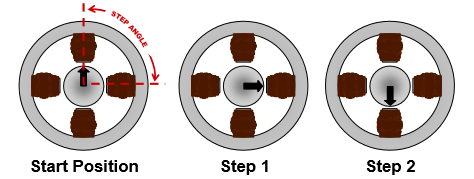
\includegraphics[width=\textwidth]{figures/move/motor1.png}
	\caption{Step Angle}
	\label{fig:angle} 
\end{figure}

Figure \ref{fig:angle} represents a stepper motor that requires 4 steps to complete a 360$^\circ$ 
rotation. This determines the step angle to be 90$^\circ$.
\newpage
The main components of a stepper motor are represented in Figure \ref{fig:main_components}, and 
they consist of stators, windings(phases), and rotor.
Attached to the output axle is the rotor, depending on the type of motor it can be magnetized.

\begin{figure}[htp]
	\centering
	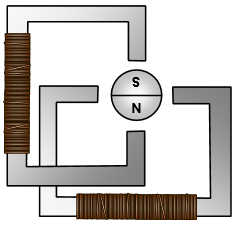
\includegraphics[width=0.3\textwidth]{figures/move/motor2.png}
	\caption{Main Components}
	\label{fig:main_components}
\end{figure}


By applying a voltage across one of the windings, current will start flowing through it. Using 
the right-hand rule, the direction of the magnetic flux can be determined. The flux will want to 
travel through the path that has the least resistance. This determines the rotor to change its 
position to minimize resistance. This is shown in Figure \ref{fig:flux}.

\begin{figure}[htp]
	\centering
	\subfloat[High Resistance]{%
		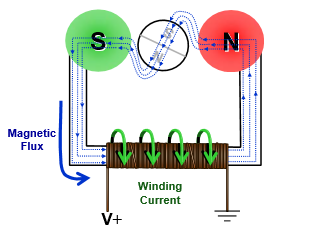
\includegraphics[width=0.4\textwidth]{figures/move/motor3.png}%
		}%
	\hfill
	\subfloat[Low Resistance]{%
		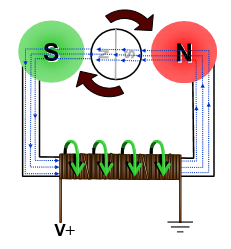
\includegraphics[width=0.4\textwidth]{figures/move/motor4.png}
	}
	\caption{Direction of Magnetic Flux}
	\label{fig:flux}
\end{figure}
\newpage
\subsection{Types of Stepper Motors}
\subsubsection{Permanent Magnet Motor}
This type of stepper motor has a magnetized rotor. Each winding will be subdivided into two, to 
better understand how to motor functions. Figure \ref{fig:bas_struct} represents the windings, and 
how they are distributed inside a stepper motor.

\begin{figure}[htp]
    \centering
    \subfloat[Rotor]{%
        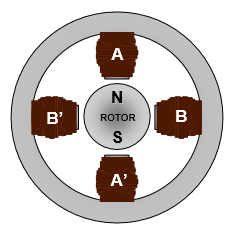
\includegraphics[width=0.4\textwidth]{figures/move/motor5.png}%
        }%
    \hfill%
    \subfloat[Winding]{%
        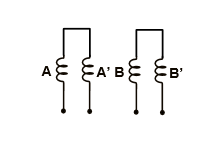
\includegraphics[width=0.4\textwidth]{figures/move/motor6.png}%
        }%
    \caption{Basic Structure of a Motor}
    \label{fig:bas_struct} 
\end{figure}

The resolution of the motor can be improved in two ways, either by increasing the number of pole 
pairs in the rotor itself, or by increasing the number of phases as shown in Figure 
\ref{fig:inc_res}.


\begin{figure}[htp]
    \centering
    \subfloat[Increased Pole Pairs]{%
        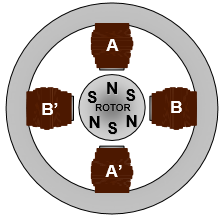
\includegraphics[width=0.4\textwidth]{figures/move/motor7.png}%
        }%
    \hfill%
    \subfloat[Increased Number of Winding]{%
        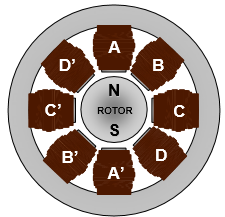
\includegraphics[width=0.4\textwidth]{figures/move/motor8.png}%
        }%
	\hfill%
	\caption{Increased resolution}
	\label{fig:inc_res}
\end{figure}

\newpage
To rotate the motor, simply apply a voltage across the windings in a sequence. A full rotation is 
shown in Figure \ref{fig:stepping_perm_magn}, with the corresponding phases energized.

\begin{figure}[htp]
    \begin{center}
    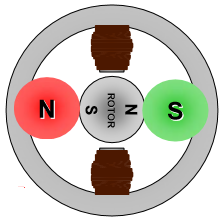
\includegraphics[width=0.2\textwidth]{figures/move/motor9.png}    
    \hfill
    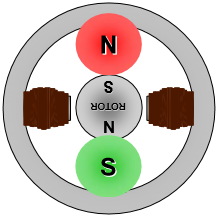
\includegraphics[width=0.2\textwidth]{figures/move/motor10.png}
    \hfill
    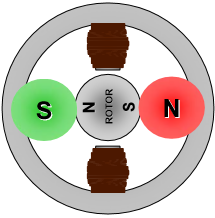
\includegraphics[width=0.2\textwidth]{figures/move/motor11.png}
  	\hfill
  	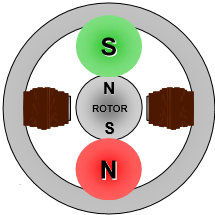
\includegraphics[width=0.2\textwidth]{figures/move/motor12.png}
    \end{center}
\end{figure}
\vspace{-10mm}
\begin{figure}[htp]
    \begin{center}
    \subfloat[$1\textsuperscript{st}$ Step]{
        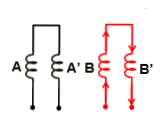
\includegraphics[width=0.2\textwidth]{figures/move/motor13.png}
        }
    \hfill
    \subfloat[$2\textsuperscript{nd}$ Step]{
        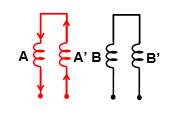
\includegraphics[width=0.2\textwidth]{figures/move/motor14.png}
        }
    \hfill
    \subfloat[$3\textsuperscript{rd}$ Step]{
    	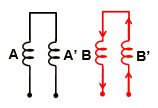
\includegraphics[width=0.2\textwidth]{figures/move/motor15.png}
    	}
  	\hfill
  	\subfloat[$4\textsuperscript{th}$ Step]{
  		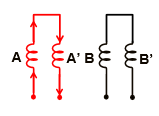
\includegraphics[width=0.2\textwidth]{figures/move/motor16.png}
  		}
  	\caption{Stepping a Permanent Magnet Motor}
  	\label{fig:stepping_perm_magn}
    \end{center}
\end{figure}
\subsubsection{Variable Reluctance Motor}
This type of motor uses a rotor that is not magnetized, and has a number of teeth as seen in 
Figure \ref{fig:var_rel_components}. The windings are configured differently, as depicted in 
\ref{fig:var_rel_components}(b), all having a common voltage source but separate ground 
connections.
They usually have 3 or 5 windings.
Greater precision can be achieved by adding more teeth to the rotor.

\begin{figure}[htp]
    \centering%
    \subfloat[Non Magnetized Rotor]{%
        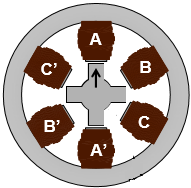
\includegraphics[width=0.3\textwidth]{figures/move/motor17.png}%
        }%
    \hfill%
    \subfloat[Windings]{%
        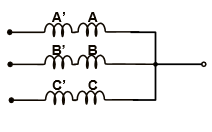
\includegraphics[width=0.4\textwidth]{figures/move/motor18.png}%
        }%
    \caption{Variable Reluctance Motor Components}%
    \label{fig:var_rel_components}%
\end{figure}
\newpage

To spin the motor, each winding is energized one at a time, and the rotor rotates to minimize 
reluctance as explained before.
Some of the differences, between this type of stepper motor and the permanent magnet motor, are 
that, in order to spin the motor in a direction, the windings have to be energized in a reverse 
sequence as opposed to the direction of the spin, as depicted in Figure \ref{fig:stepping_var_rel}.

In addition, variable reluctance motors have twice the precision of permanent magnet motors with 
the same amount of windings.
\begin{figure}[htp]
    \begin{center}
    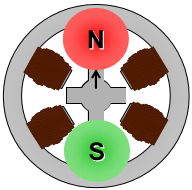
\includegraphics[width=0.2\textwidth]{figures/move/motor19.png}
    \hfill
    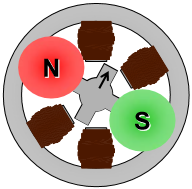
\includegraphics[width=0.2\textwidth]{figures/move/motor20.png}
    \hfill
    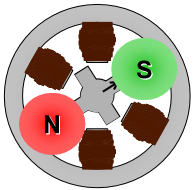
\includegraphics[width=0.2\textwidth]{figures/move/motor21.png}
  	\hfill
  	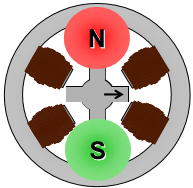
\includegraphics[width=0.2\textwidth]{figures/move/motor22.png}
	\end{center}
	\begin{center}
    \subfloat[$1\textsuperscript{st}$ Step]{
        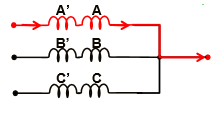
\includegraphics[width=0.2\textwidth]{figures/move/motor23.png}
        }
    \hfill
    \subfloat[$2\textsuperscript{nd}$ Step]{
        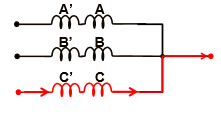
\includegraphics[width=0.2\textwidth]{figures/move/motor24.png}
        }
    \hfill
    \subfloat[$3\textsuperscript{rd}$ Step]{
    	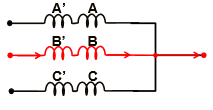
\includegraphics[width=0.2\textwidth]{figures/move/motor25.png}
    	}
  	\hfill
  	\subfloat[$4\textsuperscript{th}$ Step]{
  		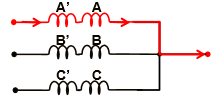
\includegraphics[width=0.2\textwidth]{figures/move/motor26.png}
  		}
  	\caption{Stepping Variable Reluctance Motor}
  	\label{fig:stepping_var_rel}
  	\end{center}
\end{figure}
\newpage
\subsubsection{Hybrid Stepper Motor}
Hybrid stepper motors borrow characteristics from both previously mentioned types.

Figure \ref{fig:hybrid_components} shows the two the main components of the hybrid stepper motor. 
On the left side, the stator can be seen consisting of 8 poles. On the right side the rotor. The 
rotor consists of two sets of teeth, corresponding to the two poles, north and south.
\begin{figure}[h]
	\centering
	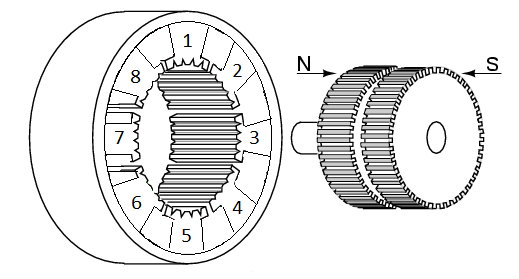
\includegraphics[width=\textwidth]{figures/move/motor27.png}
	\caption{Stator and Rotor}
	\label{fig:hybrid_components}
\end{figure}

It is important to notice two additional things. The first, is that the teeth on the rotor are not 
aligned but are interleaved. The second, is the placement of the stator teeth in respect to those 
of the rotor. Both can be observed in Figure \ref{fig:stepper}.

\begin{figure}[htp]
    \centering%
    \subfloat[Interleaved Teeth]{%
        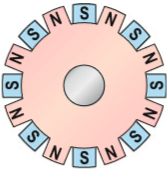
\includegraphics[width=0.4\textwidth]{figures/move/motor28.png}%
        }%
    \hfill%
    \subfloat[Stepper Motor Inside]{%
        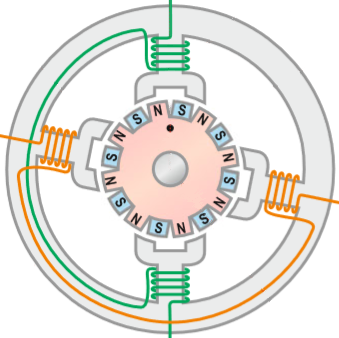
\includegraphics[width=0.3\textwidth]{figures/move/motor29.png}%
        }%
    \caption{Hybrid Stepper Motor}
    \label{fig:stepper}
\end{figure}
\newpage
Figure \ref{fig:stepper}, the windings with numbers 1 and 5 are completely aligned with the teeth 
of the rotor. Windings number 3 and 7 are completely unaligned, while the others are half aligned. 
This results in higher precision and higher torque offered by the hybrid stepper motor, depending 
on the stepping method used.

Figures \ref{fig:hybrid_first_step},  \ref{fig:hybrid_second_step}, \ref{fig:hybrid_third_step},
\ref{fig:hybrid_forth_step} 
represent the way this motor operates.

\begin{center}
	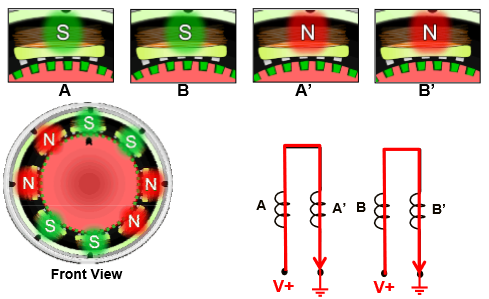
\includegraphics[width=0.8\textwidth]{figures/move/motor32}
	\captionof{figure}{First Step}
	\label{fig:hybrid_first_step}
\end{center}
By applying a voltage to both windings, the current flow can be controlled, thereby controlling the 
polarity of each stator pole, thus controlling the direction of the motor. Notice that, initially, 
poles A and A’ are completely aligned, and poles B and B’ are half aligned. 

\begin{center}
	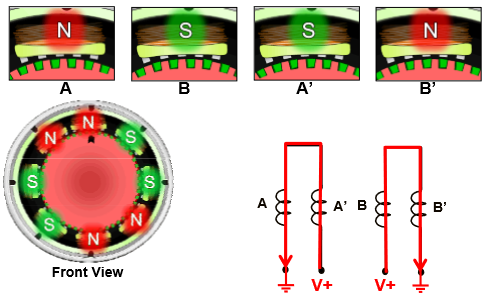
\includegraphics[width=0.8\textwidth]{figures/move/motor33}
	\captionof{figure}{Second Step}
	\label{fig:hybrid_second_step}
\end{center}

Next step involves changing the direction of the current in winding A by applying a voltage at the 
other end of the winding. Even though only the current in winding A has been changed, all stator 
poles are aligned differently. Poles A and A’ are now half aligned, and poles B and B’ are 
completely aligned.

\begin{center}
	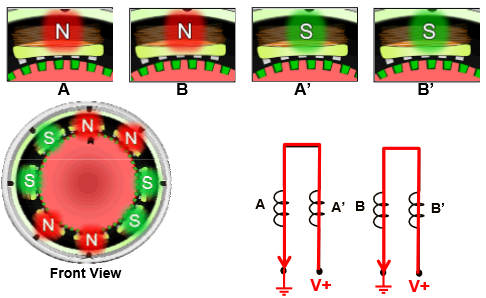
\includegraphics[width=0.8\textwidth]{figures/move/motor34}
	\captionof{figure}{Third Step}
	\label{fig:hybrid_third_step}
\end{center}

Now, changing the direction of the current in winding B, changes the polarity of the stator poles B 
and B', again, determining a change in the alignment of all stator poles. A and A’ are now 
completely aligned, and stator poles B and B’ are half aligned. The positions of the stator poles 
now correspond to those of the first step.

\begin{center}
	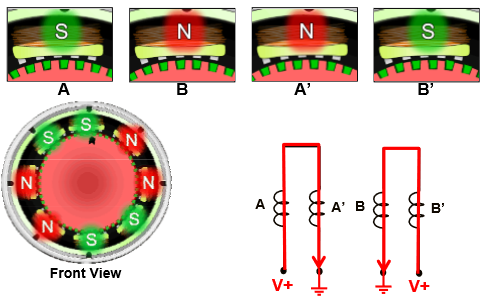
\includegraphics[width=0.8\textwidth]{figures/move/motor35}
	\captionof{figure}{Forth Step}
	\label{fig:hybrid_forth_step}
\end{center}


Finally, again changing the direction of the current in winding A, determines the rotor to move 
another step. Notice the alignment of the stator poles. A and A’ are half aligned, while B and B’ 
are fully aligned. By changing the direction of the current in winding B, the motor arrives in the 
initial state, thus repeating the sequence.


\subsection{Unipolar And Bipolar Stepper Motors}

Another classification of stepper motors, is depending on the way the windings are configured.
Even though, nowadays, almost every stepper is both.
Meaning that unipolar and bipolar, are rather modes in which the stepper motor can be driven.
Exception being, stepper motors which have only four wires coming out of them, corresponding to 
bipolar stepper motors.

Figure \ref{fig:windings} below represent the configuration of the windings in both unipolar and 
bipolar stepper motors. 


\begin{figure}[htp] 
    \centering
    \subfloat[Bipolar]{
        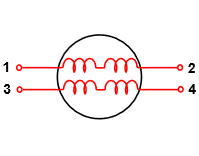
\includegraphics[width=0.4\textwidth]{figures/move/motor37.png}
        }
    \hfill
    \subfloat[Unipolar]{%
        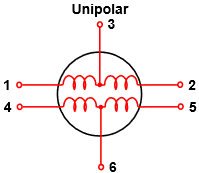
\includegraphics[width=0.4\textwidth]{figures/move/motor36.png}
        }
    \caption{Winding Configuration}
    \label{fig:windings}
\end{figure}

Bipolar stepper motors have one winding per phase. To energize the first phase, voltage needs to 
be applied to lead 1, and lead 2 needs to be connected to ground. Stepping the motor, 
involves energizing one phase, then the second, then the first phase again with reverse
polarity, meaning the voltage source and the ground must be switched between each other(lead 1 – 
ground, lead 2 – voltage source). Afterwards, the second winding is energized with reverse 
polarity. This makes driving them more difficult. We use driver boards to make the task easier. 

Unipolar stepper motors allow current flow in only one direction through the winding, unlike 
bipolar stepper motors. Because of that, a center wire has been added to each winding corresponding 
to leads 3 and 6. All the other leads are connected to ground. Outside the motor, each lead 
connected to ground is connected to a transistor first. To step the motor, apply voltage to 
the corresponding transistor to connect the lead to ground and allow current flow 
through that winding.  
\newpage
Note that the bipolar configuration as shown in Figure \ref{fig:bipolar_stepping} allows the 
current to flow in both directions, but the voltage and ground continuously switch positions. This 
makes bipolar stepper motors a bit more complicated to drive, but as previously stated, motor 
driver boards simplify the task.

\begin{figure}[htp] 
    \centering
    \subfloat[$1\textsuperscript{st}$ Step]{
        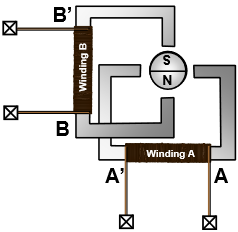
\includegraphics[width=0.3\textwidth]{figures/move/motor43.png}
        }
    \hfill
    \subfloat[$2\textsuperscript{nd}$ Step]{
        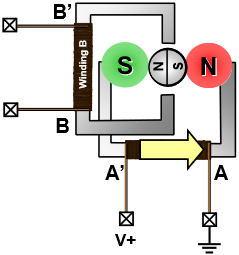
\includegraphics[width=0.3\textwidth]{figures/move/motor44.png}
        }
    \hfill
    \subfloat[$3\textsuperscript{rd}$ Step]{
    	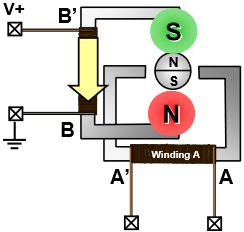
\includegraphics[width=0.3\textwidth]{figures/move/motor45.png}
    	}
   	\hfill
   	\subfloat[$4\textsuperscript{th}$ Step]{
  		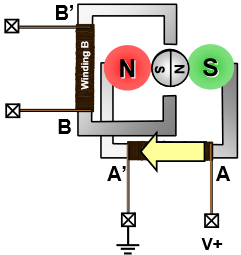
\includegraphics[width=0.3\textwidth]{figures/move/motor46.png}
  		}
  	\hfill
  	\subfloat[$5\textsuperscript{th}$ Step]{
  		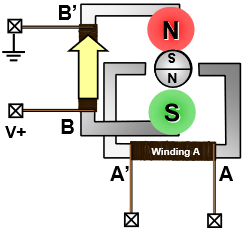
\includegraphics[width=0.3\textwidth]{figures/move/motor47.png}
  		}
  	\caption{Bipolar Motor Spinning}
  	\label{fig:bipolar_stepping}
\end{figure}
%\section{Tri-State Buffer}\label{sec:buffer}
\subsection{Motor Driver Boards}\label{sec:driver_boards}
We used motor driver boards in order to drive the motors. They provide a simple interface between 
the microcontroller and the motors, and make for a better alternative than directly driving the 
motors from the microcontroller.
\begin{figure}[htp]
	\centering
	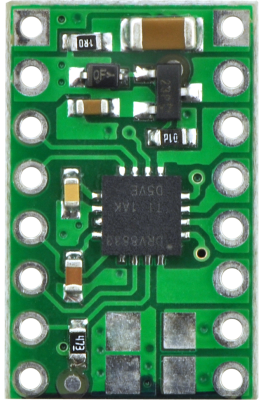
\includegraphics[scale=1,angle=90]{figures/move/driver_board}
	\caption{Driver Board}
\end{figure}
\section{Wheels}\label{sec:wheels}
The robot should be able to move in eight directions from every position.
By using traditional wheels, the robot would need to be able to steer to the desired direction, 
thus changing orientation.
This would have been a difficult task raising a number of problems.
Our solution is to use omni-wheels instead.
A standard wheel and an omni-wheel are shown in Figure \ref{fig:wheels}.

The key difference between omni-wheels and traditional wheels is their contact area.
For omni-wheels it consists of smaller wheels that are able to move freely sideways,
thus not generating any friction.

\begin{figure}[htp]
	\centering
	\subfloat[Standard Wheel]{
		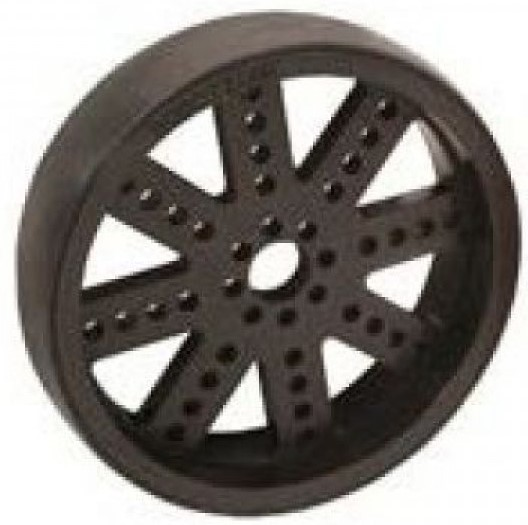
\includegraphics[width=0.2\textwidth]{figures/move/regular_wheel}
	}
	\hspace{0.2\textwidth}
	\subfloat[Omni-Wheel]{
		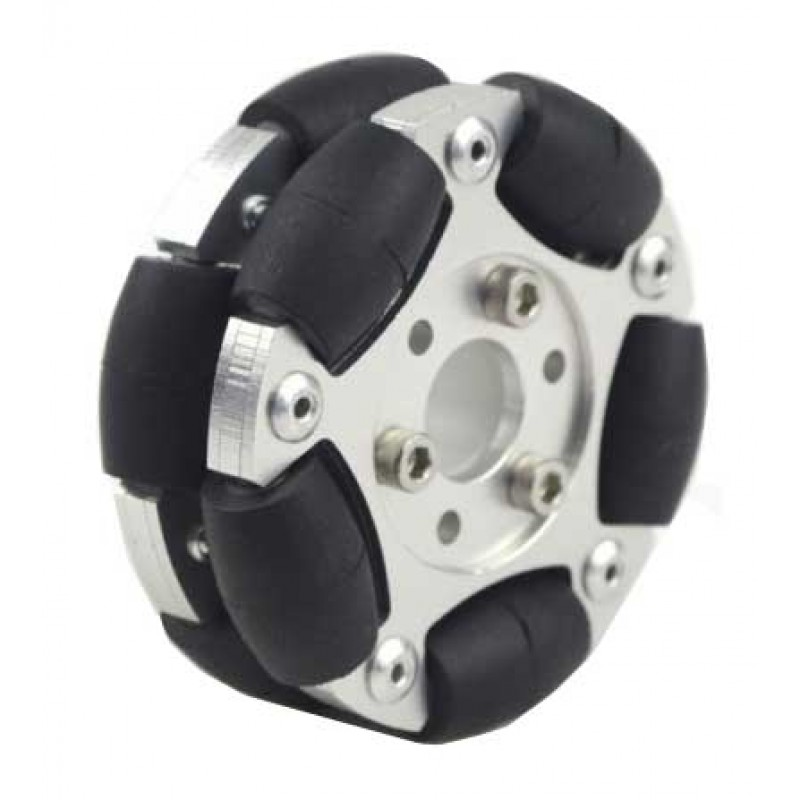
\includegraphics[width=0.2\textwidth]{figures/move/omni_wheel}
	}
	\caption{Wheels}
	\label{fig:wheels}
\end{figure}
By mounting the wheels in pairs, with the shafts crossing at a 90$^\circ$ angle, we are able to 
move the robot in any direction without needing to change the orientation of the robot.
This is achieved through rotating the pairs as shown in figure \ref{fig:forces}.
\begin{figure}[htp]
	\begin{center}
    \subfloat[North]{
    	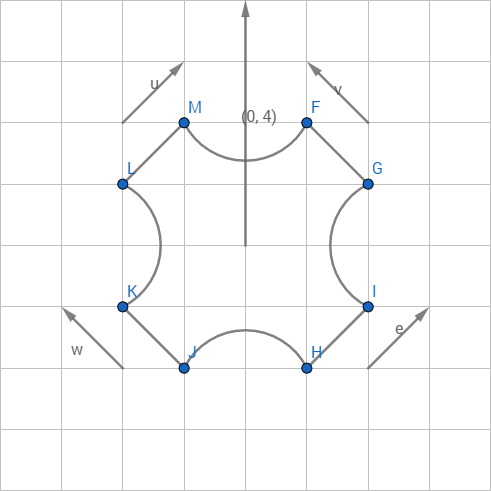
\includegraphics[width=0.2\textwidth]{figures/move/vector_addition_North}
    }
    \subfloat[East]{
    	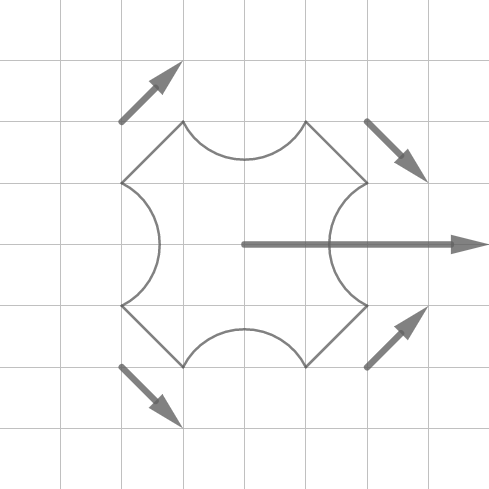
\includegraphics[width=0.2\textwidth]{figures/move/vector_addition_East}
    }
    \subfloat[South]{
   		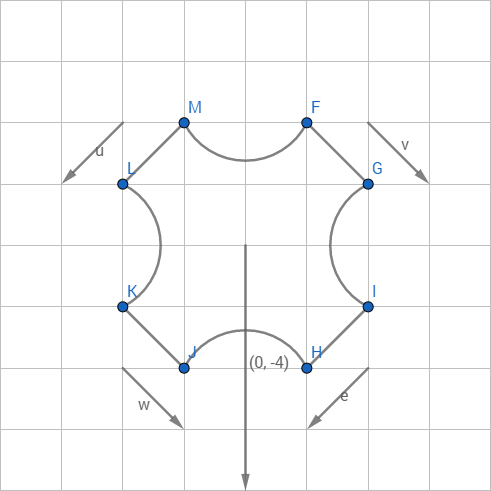
\includegraphics[width=0.2\textwidth]{figures/move/vector_addition_South}
    }
  	\subfloat[West]{
 		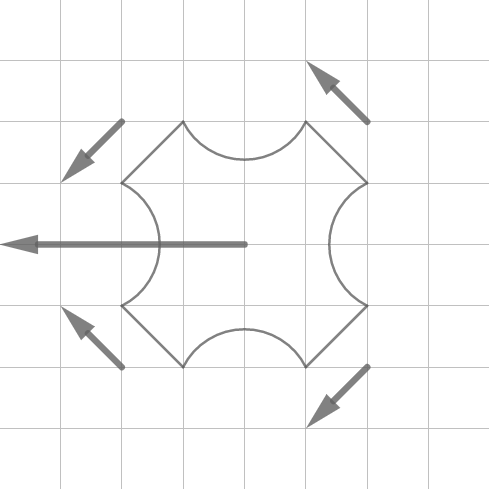
\includegraphics[width=0.2\textwidth]{figures/move/vector_addition_West}
	}
	\end{center}
	\vspace{-5mm}
	\begin{center}
    \subfloat[North-East]{
    	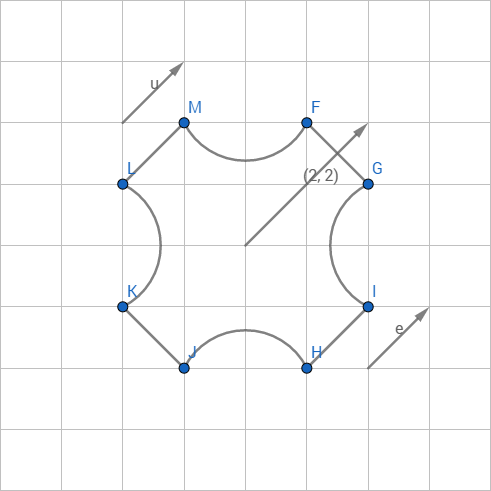
\includegraphics[width=0.2\textwidth]{figures/move/wheel_vectors_NE}
    }
    \subfloat[South-East]{
   		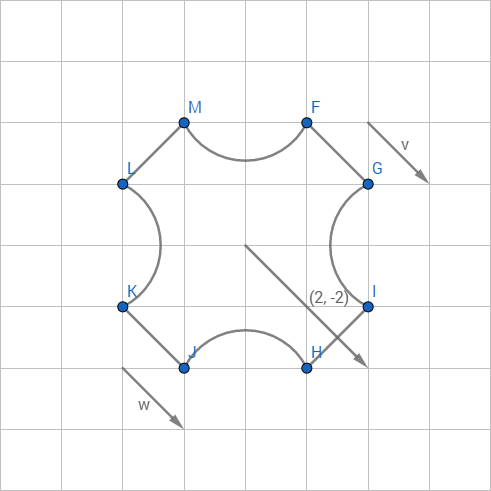
\includegraphics[width=0.2\textwidth]{figures/move/wheel_vectors_SE}
    }
    \subfloat[South-West]{
    	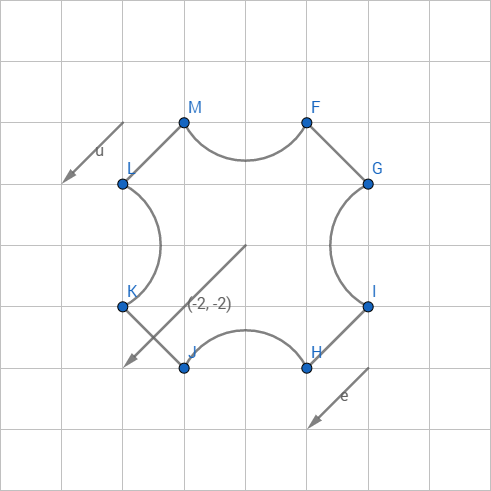
\includegraphics[width=0.2\textwidth]{figures/move/wheel_vectors_SW}
    }
  	\subfloat[North-West]{
  		\includegraphics[width=0.2\textwidth]{figures/move/wheel_vectors_NW}
	}
	\end{center}
	\vspace{-5mm}
  	\caption{Forces from Multiple Wheels Added Together}
  	\label{fig:forces}
\end{figure}
\newpage
It can also be observed that no two opposite motors spin in different directions,
because this would lead to a rotation, which is undesired for us.
This has also made our task of programming the motors more simple.
\newpage
\section{Direction Control}\label{sec:direction}
To decide the direction of the robot, we had to control which wheels turn what number of steps. 

One option would have been to control each motor individually.
This required four pins for each motor to step the motors,
and precise timing between the four motors.
Imprecise timing could introduce unintended rotation.

We decided to build our own circuit using tri-state buffers instead.
The circuit will be explained after a short explanation of tri-state buffers.

%This would drastically lower the number of pins needed, and would make for a more precise and 
%advanced way of driving the motors.

\subsection{Tri-State Buffer}
To achieve the desired movement using as few pins as possible, we decided to use Tri-State buffers.
Fewer pins make it easier to port this part of the robot to a smaller $\mu$C with fewer pins for a 
final product.

Tri-State buffers provide the possibility of disconnecting parts of the circuit, when not needed.
This allowed us to manipulate the input to the motors dynamically.

A Tri-State buffer can be thought of as a switch. Figure \ref{fig:tristate} better illustrates that 
concept.
\begin{figure}[htp]
	\begin{center}
	\subfloat[Disabled]{
		\includegraphics[width=0.3\textwidth]{figures/move/motor48}
		}
	\hspace{2cm}
	\subfloat[Enabled]{
		\includegraphics[width=0.3\textwidth]{figures/move/motor49}
		}
	\caption{Tri-State Buffer Switch Analogy}
	\label{fig:tristate}
	\end{center}
\end{figure}


When the buffer is enabled, its output corresponds to its input, either 0 or 1, "High" or "Low".
However when the buffer is a in its third state, its output is disabled, opening the circuit 
between the buffer and the next component.
That does not mean its output corresponds to a logic “Low", but instead it is in a state of high 
impedance in which the output is disconnected from the rest of the circuit.
\newpage
\subsection{Control Circuit}\label{sub:circuit}
Initially, we have thought of a movement system,
which required 16 pins to accommodate moving in all directions.
In this system we would have controlled each motor individually,
requiring 4 pins for each motor.
With this method,
it would have been necessary to have precise timing between the four stepping sequences.

Having a limited number of pins available, has forced us to think of the movement system very thoroughly.
The reason for this was that we wanted to test the movement system on the MSP430 $\mu$-C,
which only has 9 usable pins.
\todo{reference to msp}

Figure \ref{fig:mot_ctrl} shows a schematic of the motor control circuit.
\begin{figure}[htp]
	\centering
	\includegraphics[width=0.8\textwidth]{figures/move/direction_choice}
	\caption{Motor Control Circuit}
	\label{fig:mot_ctrl}
\end{figure}

The four wires coming from the microcontroller,
labeled '1', '2', '3' and '4' correspond to the stepping sequence.
They are connected to two Tri-State buffers corresponding to each pair of motors.
The location of the motors is shown in Figure \ref{fig:motor_pairs_location}.

\begin{figure}[htp]
	\centering
	\includegraphics[width=0.2\textwidth]{figures/move/Motor_pairs_location.jpg}
	\caption{Motor Pairs}
	\label{fig:motor_pairs_location}
\end{figure}

\clearpage
The first two Tri-State buffers switch the pair on or off,
dependent on it being necessary for moving in a specific direction.
The input pins, labeled ‘A Enable’ and ‘B Enable’ go to the 
two Tri-State buffers connected to each motor pair. 

Afterwards, each enabling buffer is connected to two buffers that decide the direction,
one active-high and one active-low.
Those two buffers can be controlled by one bit,
because of their opposite enable voltage.

For example, when moving North-East, only ‘Pair A’ is needed.
‘A Enable’ will have a ‘High’ signal while ‘B Enable’ will have a ‘Low’ signal.
Next, applying a ‘Low’ signal to ‘A Direction’, 
reverses the wiring of the motors determining the robot move North-East.

Note that, when moving in a specific direction,
the motors that form a pair,
have to spin in opposite directions.
One spins clockwise, while the other spins counter-clockwise.
This was achieved by wiring one motor in reverse as shown in Figure \ref{fig:reverse_wiring}.
\begin{figure}[htp]
	\centering
	\includegraphics[width=0.8\textwidth]{figures/move/motor_pairs_cedar.png}
	\caption{Motor Wiring}
	\label{fig:reverse_wiring}
\end{figure}

It is important to specify, that the robot moves in said directions using the same 
programming only by maintaining the same
orientation as in Figure \ref{fig:motor_pairs_location}.

Tables \ref{tab:directions} and \ref{tab:directions_signal} show the configurations 
required for moving in any of the eight directions.
\begin{table}[htp]
	\centering
	\caption{Directions}
	\begin{tabular}{|l|l|l|}
		\hline
		Direction 	& Pair A 	& Pair B	\\
		\hline
		North 		& forward 	& forward \\
		East 		& forward 	& backward \\
		South 		& backward 	& backward \\
		West 		& backward 	& forward \\
		\hline
		North-East 	& forward 	& off \\
		South-East 	& off 		& backward \\
		South-West 	& backward 	& off\\
		North-West 	& off 		& forward \\
		\hline
	\end{tabular}
	\label{tab:directions}
\end{table}
\begin{table}[htp]
	\centering
	\caption{Direction Signals}
	\begin{tabular}{|l|c|c|c|c|}
		\hline
		Direction & $A_{Enable}$ & $A_{Direction}$ & $B_{Enable}$ & $B_{Direction}$ \\
		\hline
		North 		& 1 & 0 & 1 & 0 \\
		East 		& 1 & 0 & 1 & 1 \\
		South 		& 1 & 1 & 1 & 1 \\
		West 		& 1 & 1 & 1 & 0 \\
		\hline	
		North-East 	& 1 & 0 & 0 & x \\
		South-East 	& 0 & x & 1 & 0 \\
		South-West 	& 1 & 1 & 0 & x \\
		North-West 	& 0 & x & 1 & 1 \\
		\hline
	\end{tabular}
	\label{tab:directions_signal}
\end{table}
\vfill
% Introduction

% ??? NEED block diagram of go()! check map? scan: yes/no? save map, move etc. (use that online code to block diagram tool)
% ??? Descripe framework in a section (see gdocs for input to block diagram) (or present at exam)
% ??? Mention we chose to focus on making our own code with the least use of finished libraries as possible, no error handling 
% ??? Mention the report will explain important aspects of out work and theoretical parts, 
%     while the finished product is a prototype and the code in the appendix
% 

% Problem / introduction?:
% - Problem and analysis:
% 	- https://en.wikipedia.org/wiki/Rescue_robot
%	- https://www.robocupgermanopen.de/sites/default/files/rescue_maze_2017.pdf
% - System diagram (what we want to build):
% Daniel has already made a nice diagram of this
% Current position should be known after each move.

% - Prototype / mechanical design / robot design (show what we wanted to to build)
% - maybe here with motor/wheels under it? chasis?
% - maybe under "problem and analysis"


% Programming Structure and Design: (try to fulfill some Akbar goals here, see those gdocs notes)
%- Robot Instruction Execution Order
%- Framework
%- Data Structure



% Robot control: (maybe after pathfinding?)
% Theory:
% - functionality
% - step/control sequence
% Implementation: (programming)
% - programming/framework etc.

% Map handling:
% Theory (how we did and thoughts):
% - Introduction (what is map handling about, what have we covered here, problems we want to solve)
% - Analysis of map input
% - Converting analog map to digital map (intro)
% - 
% Implementation:
% - Read, compare, update 

% Prototype:
% maybe something about the prototype here??
% or in conclusion at least
% read google docs



\chapter{Map Handling}
\label{ch:map_handling} % chapter label
The rescue robot should be able follow a given path from start to finish, based on a predefined map given as input.
A map provides useful information about whether areas of the map are accessible or not. 
Map data can be loaded by the robot prior to its physical presence at a location. 
Once the robot is at the starting point, it has to rely on its sensors for updated information about the surroundings. 

The map itself is a crucial part, that converted into to a graph is used by the path-finding as explained in Chapter \ref{ch:path}. 
Hence a structured way of storing the required map data for different maps was designed. 
The primary goal was make it readable by the microcontroller, but also still allow easy user input.

%Existing pathfinding algorithms such as Dijkstra and A* was studied, 
%in order to understand what input data such algorithms typically would require. 
%The pathfinding algorihtm implemented in this project is further described in chapter \ref{ch:path}.

\newpage
\section{Map Requirements}
\label{sec:map_requirements}
Maps can be found in a lot of different styles,
varying in how they represent specific informations.
Those styles often depend on the purpose of the map.
Figure \ref{sub:orient} shows a map for casual orientation purposes,
while \ref{sub:evac} shows a standardized evacuation plan.

\begin{figure}[h!tp]
    \centering
    \subfloat[Section of AAU Esbjerg]{%
        \includegraphics[width=0.4\textwidth]{figures/map/floorplan_aau.png}%
        \label{sub:orient}
        }%
    \hspace{0.1\textwidth}
    \subfloat[School layout example]{%
        \includegraphics[width=0.4\textwidth]{figures/map/floorplan_school.png}%
        \label{sub:evac}
        }%
    \caption{Examples of different maps}
    \label{fig:floor_plans}
\end{figure}
% https://www.edrawsoft.com/school-layout-example.php

Maps are often very visual, providing a lot of detailed information to the reader.
The way the information is represented differently,
makes it very hard to be interpreted automatically.
A map must provide necessary information,
in a way that can be interpreted by the micro controller.
For this project we decided that a simplified map, would be sufficient.

Table \ref{table:map_data} shows the data the map should include,
as well as some areas that have been delimited from.

\begin{table}[h!]
	\centering
	\caption{Map data}
	\begin{tabular}{|p{0.4\textwidth}||p{0.4\textwidth}|}
		\hline
		Data to be included & Data to delimit from \\ 
		\hline
		Map dimensions 		& \parbox[t]{0.4\textwidth}{Differences in height\\(levels, stairs etc.)}\\
		\hline
		Start position 		& Door openings \\
		\hline
		Finish position 	& \parbox[t]{0.4\textwidth}{Ground surface\\(slipping, traction)} \\
		\hline
		Walls 				& Objects\\
		\hline
	\end{tabular}
	\label{table:map_data}
\end{table}

\section{Map Coordinates}
\label{sec:map_coordinates} % section label
During the theoretical development we often used hand-drawn 2D maps with grids as depicted in Figure \ref{sub:2d_map}. 
The map can have a certain size and allows for an object such as a wall to have a location on the grid. 
A specific part of the map can easily be referred to by its unique coordinate in the x and y dimensions. 

For converting and storing analog maps into a usable digital representation with the same properties, 
we chose to use a 2D array as data structure. 
A 2D array can be thought of as a matrix, where a grid of numbers can be arranged in rows and columns. 
2D arrays are very similar to matrices, and differs in how elements are indexed.

The result of the different indexing methods can be seen by comparing Figure \ref{sub:2d_map} to \ref{sub:2d_array}. 
Given the same index values, the cell referred to would be different, 
as seen in Figure \ref{grid_map_vs_array}.


\begin{figure}[htp]
    \centering
    \subfloat[2D grid map]{%
        \includegraphics[width=0.45\textwidth]{figures/map/2d-map.png}%
        \label{sub:2d_map}
        }%  
    \hspace{0.05\textwidth}  
    \subfloat[2D array]{%
        \includegraphics[width=0.45\textwidth]{figures/map/2d-array.png}%
        \label{sub:2d_array}
        }%
    \caption{Difference in indexing for (3,4) in a 2D grid map and a 2D array}
    \label{fig:grid_map_vs_array}
\end{figure}
%https://i.stack.imgur.com/tFdLk.gif

Each cell in the map represents a map segment with its own set of coordinates. 
We chose to start map coordinates at zero, and had the option to switch rows and columns if needed, 
which is similar to a matrix transpose. 
This could be done in the syntax by switching i and j, 
or by switching the x and y axes when storing the map in the first place.
\\

\begin{lstlisting}[caption={Example of map segment before rows and columns are switched}]
Array: map[4][3], would give map coordinate (3,4)
\end{lstlisting}

\begin{lstlisting}[caption={Example of map segment after switching rows and columns}]
Array: map[3][4], would give map coordinate (3,4)
\end{lstlisting}

This lead to the final implementation in our program using dynamic 2D arrays, 
where the value of any given map segment easily could be accessed. 
\\
\begin{lstlisting}[caption={Example of implementation in the final code}]
Array: robot->map->segments[3][4], would return the value for map coordinate (3,4)
\end{lstlisting}
Examples of this can be seen implemented in the final code in appendix XX (some specific place?). 
\todo{fix referring to code in appendix, and code language should not be set to Python.} 
The same approach was used for handling node maps, which is further explained in Chapter \ref{ch:path}.

\newpage

\section{Map Design}
\label{sec:map_design} % section label
The grid-based map is made up of simple plain-text ASCII characters.
This makes it fairly simple and easy-to-understand, and maps can easily be created or changed by a user. 

An example of a map with 5x5 nodes can be seen in Figure \ref{sub:map_ascii}, 
where \# being walls, A being the start, B being the finish, o being nodes, and the whitespaces being open spaces. 
The same map can be seen using UTF8 encoding in Figure \ref{sub:map_utf8}. 
UTF8 has a more characters to choose from, which makes it easier to read for humans , 
while the plain-text version is easier to read for computers.

Nodes represent positions on the map where the robot can move between. 
The robot can move in any of the eight directions unless a it is blocked by a wall. 
The directions consists of four straight directions, N,E,S,W and four diagonal directions NE,SE,SW,NW. 
Nodes are explained further in Chapter \ref{ch:path}. 
\todo{explained in path chapter or in nodemap section?}

\begin{figure}[htp]
    \centering
    \subfloat[ASCII]{%
        \includegraphics[width=0.2\textwidth]{figures/map/5x5map_ascii-2.png}%
        \label{sub:map_ascii}

    }
    \hspace{0.2\textwidth}
    \subfloat[UTF8]{%
        \includegraphics[width=0.2\textwidth]{figures/map/5x5map_utf8-2.png}%
        \label{sub:map_utf8}
    }
    \caption{Example of a map with 5x5 nodes, having 11 characters per line and 11 lines.}
    \label{fig:5x5map}
\end{figure}

We found that making the map using UTF8 would require a bit more work, 
since text editors sometimes add characters to the beginning of the file. 
This is known as the byte-order-mark (BOM) which indicates the file uses UTF8 encoding. 
It also uses variable bit-length for characters, between 1-4 bytes [https://en.wikipedia.org/wiki/UTF-8].
\todo{not wikipedia PLEASE!!} 
This makes reading and storing the map to a file more complicated, which is why we chose to use plain text ASCII.

\newpage
\section{Reading Map from a File}
\label{sec:map_read} % section label %
The function {\tt map\_load} loads map data from a file and saves it in the {\tt map} struct.
Start and finish positions are read from the file as well, and saved in {\tt robot} struct.
\todo{Write about structs in the beginning of the report}

Functions were made for loading maps from a text-file, as well as saving an updated map to a text-file. 
The full code for the functions {\tt map\_load} and {\tt map\_save} can be seen in Appendix X.
\todo{fix reference}
\todo[inline]{listing showing parts of these functions}
Reading and writing maps on a computer locally, was very useful for developing and testing the map handling subsystem. 
Implementing this functionality on a microprocessor, would require it to have a file system installed.
We chose not to implement this functionality, due to the restricted time frame of this project.
As an alternative, maps can be stored directly in memory as part og the programming code. 
This solution is not as user-friendly, and updates to the map will be lost from the memory when the microcontroller is turned off.

\todo[inline]{something in between, maybe some code?}
In the C programming language the size of an array must be declared at compile time. 
The array for the map has to be large enough to hold all the map data.
Unfortunately the map size and data remains unknown until a map is loaded, which happens at runtime.

One way of dealing with this, is by using a 2D array with a fixed size, large enough to store maps of a convenient size. 
We chose to use a dynamic 2D array instead. 
This more advanced approach would give us more experience, by using dynamic memory allocation and pointers to implement this solution in the application.

The required size of the dynamiic 2D array can be calculated by counting the lines and characters of the map,
which is equivalent to the rows and columns needed for the array.
A map with 5x5 nodes will have 11 characters in each line and a total of 11 lines,
as illustrated in Figure \ref{fig:5x5map}.
To store the map, an 11x11 2D array is required.
Now that the required array size is known, it can be allocated in the memory.\\
\todo[inline]{insert code}
- Example of allocating 2d array\\
- putting data in 2d array ???\\


ORDER:\\
map load\\
hex values\\
node map load\\
scan\\
map save\\
\todo{ORDER can be removed now I think}


\section{Encoding Walls in a Single-byte Value}
\label{sec:map_hex} % section label
Each node in the map potentially has up to eight neighbour nodes. 
The robot can move to any of the neighbour nodes, unless it is blocked by a wall, as illustrated in Figure \ref{fig:node_move_directions}.
\todo{insert figure of a node and 8 arrows}


To represent the possible directions to move in, we decided to use the boolean values 0 and 1. 
Here 0 would mean it is possible to move that direction to the neighbour node, while 1 means the direction is blocked by a wall.

Since each 0 or 1 can be represented by one bit, it is possible to store data about all eight directions in a single byte.
byte --> [0000 0000]
\todo{insert figure or table here as an example?}

Depending on the individual bits, the byte will have a certain value.
Since all values are stored as binaries in the memory, a hexadecimal representation was often used in the programming.

\todo{merge this section with Daniels 5.7 Implementation?}

\section{Building a Node Map}
\label{sec:map_node} % section label
Path finding algorithms operate with a special type of map called a graph.
A graph consists of only nodes and edges, as explained more in detail in Section \ref{sec:graphs}.
The function {\tt node\_map\_load} converts the ordinary map made of ASCII characters, into a map that only consists of nodes.

Like with linked lists, {\tt structs} can be used as a data structure to store data of different types. 
\todo{refer to structs in appendix?}
To store the node map we created the data structure {\tt Nodes struct} to hold all the necessary data for the individual nodes.
Each {\tt Nodes struct} has pointers to the eight neighbour {\tt node structs}.
This is similar to the principle of having a pointer in a linked list pointing to the next element.
\todo{insert node struct code here showing the node struct?}

A dynamic 2D array gets filled with {\tt Nodes struct}, one for each node in the map. 
\todo{code here?}
A pointer to the declared 2D array gets stored in the {\tt robot struct}.
This allows for easy access to all the data for a given node, just by using the nodes position on the map as the array index values.

\todo{give example}
robot->nodemap.node[i][j].[name of element in nodes struct]

\section{Map Validation Using Sensors}
\label{sec:map_check} % section label
There might be rescuing scenarios where parts of the map, or even the entire map, would be unknown.
External factors such as an explosion in a building, could also change the surroundings dramatically, making the map data invalid.
 
The robots current location on the map is known at all times. 
After the robot has moved to the next node on the map, its current position is updated.
At the robots current location, sensors scans the surrounding environment for walls in the eight possible move-directions.
The feedback from the sensors is returned as a single-byte value, as described in Chapter \ref{ch:scan}.

The single-byte from the {\tt scan} function gets compared to the single-byte in the map array, for the robots current location.
If changes to the surroundings are detected, the 2D map array gets updated and saved to the text-file.
\todo{insert code where char map gets updated based on the scan return and robots current position}

Every time a change in the map is detected, the pathfinding function is called
\todo{insert function name or code}. 
This calculates the most efficient path from the robots current location to the finish, using the updated map data. 
\todo{insert code from map-check function here}
\todo{it could maybe be used somewhere else to explain what the robot does, if not just leave it here.}

\section{Writing Map to a File}
\label{sec:map_save} % section label
Sensors scan the surroundings for walls, at the robots current position.
If changes are detected, the map gets updated as described in Section \ref{sec:map_check}.

If the updated map is kept only in memory, it will be lost once the microcontroller is turned off, since this is not a persistent storage. To prevent this during testing, the map was saved in a text-file.

The individual map segments that consists of ASCII characters, gets written to the map text-file.
This is done by iterating through the entire 2D map array.

\todo{map\_save code}


\chapter{Scan}\label{ch:scan}
In an attempt to take it a step further\note{be more specific please - maybe, To check if the map matches the real physical environment...}, we decided to use IR distance sensors. 
Initially, our robot is supposed to find the 
shortest path from A to B, on a map. 
In rescue situations, often, the map provided does not match 
the actual outline, possibly due to different events that 
altered the outline, such as wall collapses, that might 
obstruct the movement in a certain direction.

By using 8 IR sensors, we can detect changes in all directions 
the robot can move in. If a change is detected, this will be
accounted for in the maphandling code.

\todo{do we mention the range of the sensors and how they work? And the actual distance we have to move in a single step??}

\section{Sensor}\label{sec:sensor}
For detecting any changes in the outline of the map, we have 
used analog IR sensors. Our first idea was to use digital
sensors, but unfortunately we couldn't find any. Using analog sen
\chapter{Pathfinding}\label{ch:path}
Pathfinding is generally the process of finding a path from a given starting point ('A')
to a given destination ('B'),
on a given map.

There are different approaches to find the best path,
and different qualifiers for 'best'.

We chose to define 'best' as 'shortest time',
because in a real world application time is the most crucial resource in rescue.
In other applications 'best' could also mean shortest distance, least expensive (toll roads),
most convenient or any number of other qualifiers.

Since our robot has approximately equal movement speed in all used directions,
the shortest distance path will be very close to the shortest time path.
Since our robot only operates on a very limited map,
the shortest distance was also easiest to evaluate.

We chose to start implementing Dijkstra's shortest path algorithm,
since it is fairly simple to understand
and can be used as a baseline for better, more complicated algorithms,
like A*.

\section{Dijkstra}
Like with many others,
is the first step in Dijkstra's algorithm to reduce the map to the necessary minimum.
After this reduction, the map only consists of \emph{nodes} and \emph{edges}.
An edge connects two nodes together and has one integer \emph{travel cost}.
In this integer is stored how much it costs to traverse along that edge,
measured in the metric that should get optimized (in our case distance).

A node has a \emph{name}, an integer \emph{travel cost} and a reference to another node \emph{parent}.
The name is used as an identifier


\cite{Madsen2010}, \cite{Oetiker2010} and \cite{Mittelbach2005}.
\missingfigure{We need a figure right here!}
\chapter{Conclusion}\label{ch:conclusion}
In case you have questions, comments, suggestions or have found a bug, please do not hesitate to contact me. You can find my contact details below.
  \begin{center}
    Jesper Kjær Nielsen\\
    \href{mailto: jkn@es.aau.dk}{jkn@es.aau.dk}\\
    \href{http://kom.aau.dk/~jkn}{http://kom.aau.dk/\textasciitilde jkn}\\
    Fredrik Bajers Vej 7\\
    9220 Aalborg Ø
  \end{center}

\printbibliography[heading=bibintoc]
\label{bib:mybiblio}
\appendix
\chapter{Appendix A name}\label{ch:appAlabel}
Here is the first appendix

\end{document}
